\documentclass[14pt]{extarticle}
\usepackage{circuitikz}
\usepackage{geometry}
\usetikzlibrary{arrows}
\usepackage{parskip}
\geometry{left=2cm,right=2cm,top=1cm,bottom=2cm,includeheadfoot}
\usepackage[cmintegrals,cmbraces]{newtxmath}
\usepackage{ebgaramond-maths}
\usepackage[T1]{fontenc}
\usepackage{siunitx}
\usepackage{pdfpages}
\usepackage[tiny]{titlesec}
\usepackage{tabularx,booktabs}
\newcolumntype{Y}{>{\centering\arraybackslash}X}
% \usepackage{hyperref}
% \hypersetup{
%     colorlinks=true,
%     linkcolor=blue,
%     filecolor=magenta,      
%     urlcolor=blue,
% }


\pagestyle{empty}
\renewcommand{\frac}{\dfrac}


\begin{document}
\noindent  
\large \textbf{Physics of Wave and Oscillation} \smallskip \newline
Assignment 3 \bigskip \newline
\small Written on \today \medskip
\hrule
\bigskip
\section{System Equation of Driven RLC Circuit}
\begin{center}
    \begin{circuitikz}[american, scale = 1.25][american voltages]
        \draw (0,0)
          to[sV = $v_{in}$] (0, 2) % The voltage source
          to[R, v^<=$v_R$] (3,2) % The resistor
          to[C, v^<=$v_C$] (3,0) % Capacitor
          to[L, v^<=$v_L$] (0,0); % Inductor
          \draw[thin, ->, >=triangle 45] (1.5,1)node{$i$}  ++(-60:0.5) arc (-60:220:0.5);   
          \end{circuitikz}
\end{center}

Consider RLC circuit where the three components are all in series with the voltage source. The direction of voltage and current between each component are assumed to be like in the figure. We will derive the differential equation of the system starting from the Kirchhoff's Voltage Law:
\begin{align}
    v_R + v_L + v_C = v_{in}
\end{align}
First we analyze each element of the circuit below: 
\begin{itemize}
    \item For $R$: $v_R = iR$.
    
        \begin{circuitikz}[american voltages]
            \draw (0, 0) to [R, v^<=$v_R$, f_<=$i$] (2.5,0);
        \end{circuitikz}

    \item For $C$: $\frac{C dv_C}{dt} = \frac{dq}{dt} = i$, where $q$ is the electrostatic charge of the capacitor. By Coulomb's Law, we have $q = v_C C$. The instant change of $q$ is equal the current that passes through the capacitor. 
    
        \begin{circuitikz}[american voltages]
            \draw (0, 0) to [C, v^<=$v_C$, f_<=$i$] (2.5,0);
        \end{circuitikz}

    \item For $L$: $v_L = \frac{d\phi}{dt} = L\frac{di}{dt}$, where $\phi = Li$ is the magnetic flux through the coil. By Faraday's law of induction, the voltage will be induced in a way that hindered the change in magnetic flux through the circuit. If we assume the positive sign of voltage and direction of current like in the figure, the positive change of current will induce a voltage with the assumed sign that hinders the current source. 
    
        \begin{circuitikz}[american voltages]
            \draw (0, 0) to [L, v^<=$v_L$, f_<=$i$] (2.5,0);
        \end{circuitikz}
\end{itemize}
We let $v_{in}$ be the typical sine wave input: $E_0\cos \omega t$. To obtain a differential equation in terms of $q$, we substitute $v_L = L\frac{di}{dt} = L\frac{d^2q}{dt^2}, v_R = R\frac{dq}{dt}, v_C = \frac{1}{C}q $ into (1):

\begin{align*}
    L\frac{d^2q}{dt^2} + R\frac{dq}{dt} + \frac{1}{C}q &= E_0 \cos(\omega t)\\
    \frac{d^2q}{dt^2} + \frac{R}{L}\frac{dq}{dt} + \frac{1}{LC}q &= \frac{E_0}{L} \cos(\omega t)\\
\end{align*}
Let \[\frac{1}{\sqrt{LC}} = \omega_0 , \frac{R}{L} = 2\gamma,\] we obtain a familiar differential equation:
\begin{align}
    \frac{d^2q}{dt^2} + 2\gamma\frac{dq}{dt} + \omega_0^2 q = \frac{E_0}{L} \cos(\omega t)
\end{align}

The equation for a series RLC circuit and a spring pendulum looks really similar. We will attempt to create an analogy table to map between the two system. 

\begin{tabularx}{\textwidth}{c *{4}{Y}}
    \toprule
    \multicolumn{2}{c}{Spring Pendulum} & \multicolumn{2}{c}{RLC Circuit}  \\ \hline
    \midrule
    Displacement & $x$ & Charge & $q$ \\
    Damping & $\Gamma$ & Resistance & $R$ \\
    Mass & $m$ & Inductance & $L$ \\
    Compliance & $1/k$ & Capacitance & $C$\\
    Force & $F$ & Voltage & $E_0$  \\  
    Velocity & $v$ & Current & $i$  \\
    Momentum & $p = mv$ & Flux & $\Phi = Li$  \\
    \bottomrule
\end{tabularx}



\section{Solution to the System Equation}

By following the lectures, we have known that there are three steps to solve the differential equation: 
\begin{itemize}
    \item Find the homogeneous solution \(q_{H}(t)\) 
    \item Find the particular solution \(q_{P}(t)\)
    \item The total solution is then the sum of the homogeneous solution and the particular solution as follows  
    \[q(t)=q_{\mathrm{H}}(t)+q_{\mathrm{P}}(t)\]
\end{itemize}
The homogeneous solution would have three different forms: 
\begin{itemize}
\item \(\gamma<\omega_{0} \quad \Rightarrow \quad\) under-damped dynamics:
$q_H = A e^{-\gamma t} \cos (\sqrt{\omega_{0}^{2}-\gamma^{2}} t+\alpha)$.  
\item \(\gamma=\omega_{0} \quad \Rightarrow \quad\) critically-damped dynamics:
$q_H = x(t)=(a t+b) e^{-\gamma t}$ 
\item \(\gamma>\omega_{0} \quad \Rightarrow \quad\) over-damped dynamics:
$q_H = e^{-\gamma t}\left(R_{1} e^{+\sqrt{\gamma^{2}-\omega_{0}^{2}} t}+R_{2} e^{-\sqrt{\gamma^{2}-\omega_{0}^{2}} t}\right)$ 
\end{itemize}

Similar to the spring pendulum, the particular solution is:
\begin{align*}
    q_P = Q \cos(\omega_0 - \beta)
\end{align*}
where 
\begin{align*}
    Q &= \frac{E_0/L}{\sqrt{(\omega_0^2  - \omega^2)^2 + 4\gamma^2\omega^2}} \\
    \beta &= \arctan(\frac{2\omega_0\gamma}{\omega_0^2 - \omega^2}) 
\end{align*}
The homogeneous term will fade out as time passes. The second term of particular solution will last as long as there is the external voltage. Just for fun we will include here a graph of a driven RLC circuit with $E_0 = 5 \si{V}, f = 10 \si{kHz}, R = 500 \si{\ohm}, L = 1 \si{H}, C = 1 \si{\mu C} $.  

\begin{figure}[h]
    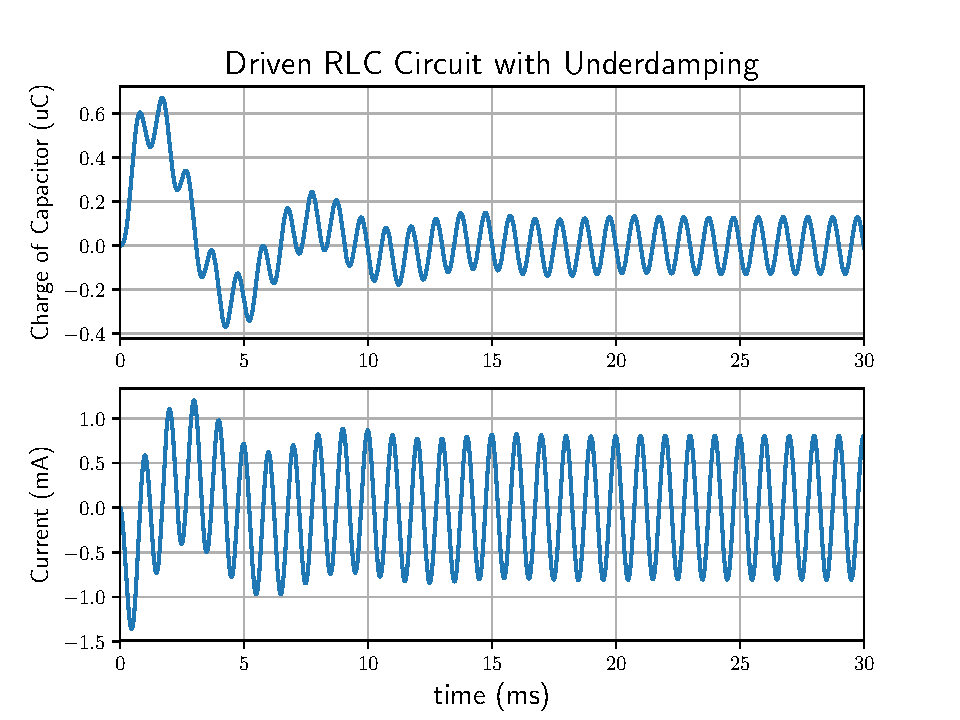
\includegraphics[width=150mm,scale=0.5]{test}
\end{figure}

We would like to make some adjustment to A and $\beta$ to match with convention in circuit theory.
\begin{align*}
   Q &= \frac{E_0/L}{\sqrt{(\omega_0^2  - \omega^2)^2 + 4\gamma^2\omega^2}} \\
   &=  \frac{E_0}{L\sqrt{(1/LC  - \omega^2)^2 + \omega^2(R/L)^2}} \\
   &=  \frac{E_0}{\omega\sqrt{((1/\omega C)  - \omega L)^2 + R^2}} \\
   &=  \frac{E_0}{\omega\sqrt{(Z_L  - Z_C)^2 + R^2}} \\
   &= \frac{E_0}{\omega Z} \\
   \beta &= \arctan(\frac{2\omega_0\gamma}{\omega_0^2 - \omega^2})  \\
   &= \arctan(\frac{R}{1/\omega C - \omega L}) \\
   &= \arctan(\frac{R}{Z_C - Z_L}) 
\end{align*}

The quality $Z_C$ and $Z_L$ are called the impedance of capacitor and inductor respectively, whereas $Z$ is called the impedance of the circuit. It consists of a resistance and $R$ a reactance $Z_L - Z_C$. Why should we denote this way? Let's check the current:

\begin{align}
    i = \frac{dq}{dt} = A\omega \cos(\omega_0 - \beta + \pi/2) = \frac{E_0}{Z}\cos(\omega_0 - \beta + \pi/2) = I_0\cos(\omega_0 - \beta + \pi/2)
\end{align}

Later in other part of our derivation, we may see more convenient points of this denotation. \newline
On the other hand, we would like to think about the complex plane a bit. We could remember from the previous lectures, $Q$ is the real part of a complex number $q*$, which came from the solver to find $q(t)$:
\begin{align*}
    q*\left(-\omega^{2}+2 \gamma j \omega+\omega_{0}^{2}\right) e^{j \omega t}=\frac{E_0}{L} e^{j \omega t} 
\end{align*}

We will use $j$ instead of $i$ to denote the complex part. Now, for purely reason of convention, we would like inspect the current element $i$ by differentiate the above equation in term of time:
\begin{align*}
    q^{*} a\left(-\omega^{2}+2 \gamma j \omega+\omega_{0}^{2}\right) \omega j e^{j \omega t}&=j\omega \frac{E_0}{L} e^{j\omega t}\\ 
   i^{*}\left(-\omega^{2}+2 \gamma j \omega+\omega_{0}^{2}\right) e^{j \omega t}&=j\omega \frac{E_0}{L} e^{j\omega t} 
\end{align*}
Now we could write $i*$ in terms of $R, Z_C, Z_L$:
\begin{align*}
   i^{*} &=\frac{j \omega E_0/L}{\left(-\omega^{2}+2 j\gamma  \omega+\omega_{0}^{2}\right)} \\
   &= \frac{j\omega  E_0}{L(1/LC -\omega ^2) + j\omega R} \\
   &= \frac{E_0}{j(Z_L -Z_C) + R} \\
   &= \frac{E_0}{Z^*}
\end{align*}
We could then obtain
\begin{align*}
    I_0 &= \frac{E_0}{\sqrt{(Z_L  - Z_C)^2 + R^2}} \\
    \beta &= \arctan(\frac{R}{Z_C - Z_L}) 
\end{align*}
from just some observation in the complex plane. \newline
We have $Z^*=r_1e^{j\phi_1}$ and $1/Z^*=r_2e^{j\phi_2}$. But $Z^*(1/Z^*) = 1$ so $r_1 = 1/r_2$ and $\phi_1 = -\phi_2 = -\beta + \pi/ 2 $. We could find $I_0$ and $\beta$ without much calculation. 
\begin{center}
\begin{tikzpicture}[>=latex]
    \draw[style=help lines] (0,0) (3,2);
    
    \coordinate (vec1) at (300:2); 
    \coordinate (vec2) at (60:4);
    \coordinate (vec3) at (0:3.5);
    \coordinate (vec4) at (90:3.5);
    \coordinate (vec5) at (270:3.5);
    \coordinate (vec6) at (180:3.5);
    
    \draw[->,thick,black] (0,0) -- (vec1) node[right] {$1/Z*=r_2e^{j\phi_2}$};
    \draw[->,thick,black] (0,0) -- (vec2) node[below right] {$Z^* = j(Z_L-Z_C) + R = r_1e^{j\phi_1}$};
    \draw[->,thick,black] (0,0) -- (vec3) node [below] {$Re$};
    \draw[->,thick,black] (0,0) -- (vec4) node [left] {$Im$};
    \draw[->,thick,black] (0,0) -- (vec5);
    \draw[->,thick,black] (0,0) -- (vec6);
    
    \draw [red, thick] (1.0,0) arc [start angle=0, end angle=60, radius=1cm]
        node [midway, right] {$\phi$};    
    
    \draw [blue, thick] (0.75,0) arc [start angle=0, end angle=-60, radius=0.75cm]
        node [midway, right] {$-\phi$};    
    \end{tikzpicture}
\end{center}

\section{Energy State in Driven RLC Circuit}
Let's analyze the RLC energy state like in a spring pendulum system. As we already mapped the elements of the mechanical system to the electrical system, we could actually deduce the corresponding energy also:  

\begin{tabularx}{\textwidth}{c *{4}{Y}}
    \toprule
    \multicolumn{2}{c}{Spring Pendulum} & \multicolumn{2}{c}{RLC Circuit}  \\ \hline
    \midrule
    Energy supplied & $E=\int Fudt$ & Energy supplied & $E = \int vidt$ \\
    Power supplied & $P = Fu$ & Power supplied  & $P =vi$ \\
    Power by damper& $P = u^2 \Gamma$ & Power by resistor& $P = i^2 R$ \\
    Kinetic energy& $E= M u^{2}/2$ & Conductor's magnetic energy & $E= L i^{2}/2$\\
    Potential energy& $E= kx^2/2$ & Capacitor's electrostatic energy & $E= q^2/2C $  \\  
    \bottomrule
\end{tabularx}

The energy in the capacitor at time t is:
\[
    w_C = \frac{q^2}{2C} = \frac{E_0^2}{2C \omega^2 Z^2}\cos(\omega t - \beta)^2 
\]
The energy in the inductor at time t is:
\[
    w_L = \frac{1}{2}Li^2 = \frac{L E_0^2}{ 2Z^2}\sin(\omega t - \beta)^2
\]

The total energy is the sum
\begin{center}

\begin{align*}
    w &= w_C + w_L = \frac{E_0^2}{2Z^2 \omega}(\frac{1}{\omega C}\cos(\omega t - \beta)^2  + \omega L\sin(\omega t - \beta)^2)  \\
    &= \frac{E_0^2}{2Z^2 \omega}(\frac{1}{\omega C}\cos(\omega t - \beta)^2  + \omega L - \omega L \cos(\omega t - \beta)^2) \\
    &= \frac{E_0^2}{2Z^2 \omega} (\omega L + (\frac{1}{\omega C} - \omega L)\cos(\omega t -\beta)^2) \\
    &=  \frac{E_0^2}{2Z^2 \omega} (Z_L + (Z_C - Z_L)\cos(\omega t -\beta)^2) \\
    (&= \frac{1}{2} L\omega^{2} A^{2}+\frac{1}{2} L(\omega_{0}^{2}-\omega^{2}) A^{2} \cos ^{2}(\omega t-\beta) )
\end{align*}
    
\end{center}

As the voltage varies with time, the instant energy state is also a function of time. We will find the average energy through a cycle:
\begin{align*}
    W &= \frac{1}{T}\int_0^{T}\left\{\frac{E_0^2}{2Z^2 \omega} (Z_L + (Z_C - Z_L)\cos(\omega t -\beta)^2)\right\} \\
    &= \frac{E_0^2(Z_L+Z_C)}{4Z^2\omega} = \frac{E_0^2(Z_L+Z_C)}{4Z^2} \frac{T}{2\pi}\\
    (&= \frac{1}{4}\left(\omega_{0}^{2}+\omega^{2}\right) L A^{2})
\end{align*}
We see that the average energy in every cycle is a constant. In the steady state, similar to a spring pendulum, the work $W_X$ generated by the voltage  will be transferred into heat $W_R$ by the resistor. We will show that $W_R$ and $W_X$ are equivalent. 
\begin{align*}
    W_X &= \int_0^T v_{in} i dt = \int_0^T E_0 \cos(\omega t) \frac{E_0}{Z} (-\sin(\omega t-\beta)) dt\\
    &=  \frac{E_0^2}{Z} \int_0^T\cos\omega t (- \sin\omega t\cos\beta + \sin\beta \cos\omega t) dt \\
    &=  \frac{E_0^2}{2Z} T \sin\beta  \\
    (\sin\beta &= \frac{R}{\sqrt{R^2 + (Z_L-Z_C)^2}} = \frac{R}{Z}) \\
    W_R &= \int^T_0 i^2 R dt= \int^T_0 \frac{E_0^2R}{Z^2}\sin^2(\omega t - \beta) dt\\
    &= \frac{E_0^2 R}{2Z^2} T = \frac{I_0^2R}{2} T\\
\end{align*}

\section{Resonance Phenomenon}

Let's calculate the power of the voltage:
\[
\bar{P}=\frac{\Delta W_{X}}{\Delta t}
\]
As we already got the amount of work in a cycle of T, the power is simply:
\[
\bar{P}=\frac{E_0^2 R}{2Z^2} = \frac{E_0^2 R}{2(R^2 + (Z_L-Z_C)^2)} 
\]

In the above equation, we can see that only the term $(Z_L-Z_C)^2$ is dependent of $\omega$. The power would reach maximum value if: 
\[ Z_L=Z_C \quad \text{ or } \quad \omega = \omega _0\] 
And in other cases of $\omega \rightarrow \infty \text{ and } \omega \rightarrow 0; \quad \bar{P} \rightarrow 0$. The maximum power is:
\[
\bar{P}_{\max }=\frac{E_0^{2}}{2 R}
\]
At a certain frequency the power dissipated by the resistor is half of the maximum power which as mentioned occurs at \(\omega = \omega_{0}\) The half power occurs at the frequencies for which:
\begin{align*}
\frac{1}{\sqrt{2}}=\frac {R}{Z} = \frac{ R }{\sqrt{\left(Z_L - Z_C\right)^{2}+(R)^{2}}} 
\implies \pm R = \omega L - \frac{1}{\omega C}
\end{align*}
The equation has two roots: 
\begin{align*}
    \omega_{1} &=-\frac{R}{2 L}+\sqrt{\left(\frac{R}{2 L}\right)^{2}+\frac{1}{LC}} \\
    \omega_{2} &=\frac{R}{2 L}+\sqrt{\left(\frac{R}{2 L}\right)^{2}+\frac{1}{LC}}
\end{align*}
where \(\Delta \omega = \omega_{2} - \omega_{1} = 2\gamma\) is the bandwidth, \(\omega_{1}\) is the lower half-power frequency and \(\omega_{2}\) is the upper half-power frequency. By multiplying the two roots we also realize that $\omega_{0}=\sqrt{\omega_{1} \omega_{2}}$. \newline
The resonance phenomenon and bandwidth is applied into filtering in electrical engineering. The rapid change in impedance near resonance can be used to pass or block signals close to the resonance frequency.
\end{document}